\documentclass[conference]{IEEEtran}
\ifCLASSINFOpdf
  \usepackage[pdftex]{graphicx}
\else
  \usepackage[dvips]{graphicx}
\fi

\usepackage[cmex10]{amsmath}
\usepackage{algorithmic}
\usepackage{algorithm}
\usepackage{array}

\ifCLASSOPTIONcompsoc
  \usepackage[caption=false,font=normalsize,labelfont=sf,textfont=sf]{subfig}
\else
  \usepackage[caption=false,font=footnotesize]{subfig}
\fi
\usepackage{fixltx2e}
\usepackage{stfloats}
\usepackage{url}
% correct bad hyphenation here
\hyphenation{op-tical net-works semi-conduc-tor}

\begin{document}
\title{Programming Assignment 4: Vector Addition \\ Continued}

\author{\IEEEauthorblockN{Luke Fraser}
\IEEEauthorblockA{Computer Science Department\\
University of Nevada, Reno\\
Email: Luke.Fraser.A@gmail.com}}

\maketitle

\begin{abstract}
Vector addition is a simple problem in computing that is typically done in a sequential fashion. An N-sized vector array is summed up to compute it total sum. The sequential implementation is very slow when N gets large. As well this type of problem well suited for parallel execution. In this assignment vector addition is taken one step further by allowing arbitrary thread and block sizes as well as GPU recursive behavior and CPU hand-offs for when sequential outperforms parallel. This implementation was also tested more rigorously at different sizes of N.
\end{abstract}

\IEEEpeerreviewmaketitle

\section{Introduction}
The previous assignment had far less strict guidelines on the vector addition implementation. The product that was produced was a kernel function that operated on even numbered sizes of N. As well the block and thread sizes were dependent on the size of N to an extant. Being that they had to multiply to $N/2$.

The kernel function was similar to an implementation on the Nvidia documentation. The kernel initially sum two adjacent values of the source vector by each thread in a block. This divides the problem by 2. This is the first reduction. The second reduction loops over a $2^n$ sized array in shared memory further reducing the summation until the total for the particular block is obtained. The kernel result is a block wise reduction. After running the kernel once the size of the resulting vector is equivalent to the number of blocks.

There were two central issues with this implementation:
\begin{itemize}
  \item \textbf{Dependency}: In order for every part of N to summed the number of $blocks*threads=\frac{N}{2}$. The implications of this being that blocks and threads were calculated and could not be arbitrary set for a given value of N.
  \item \textbf{Thread = $2^n$}: For the result to be correct the number of threads had to be a power of 2. This was due to how the warp reductions occurred. A low cost bit-shift was used to hand the final reductions. This only worked when the threads size was a power of 2.
  \item \textbf{CPU Recall}: The original kernel in order to finish the reduction into a final sum needed to be called several times by the CPU. Each reduction would only shrink the problem down to the number of blocks. In order to finish the problem the resulting vector would have to be passed as the source vector to be shrunk further.
\end{itemize}

The original kernel needed to be augmented in order to handle the new constraints.
\section{Implementation}
The original kernel was augmented to achieve the new requirements of the programming assignment. The final implementation featured two new versions of the algorithm. One version that was recalled by the CPU and another that was recalled by itself. Algorithm~\ref{alg:original} shows the original implementation of the vector addition. Algorithm~\ref{alg:original} implementation was limited mainly by the shared memory size and warp wise reduction step. This is evident in the \emph{FOR loop} where $s$ is bit shifted at each iteration. By doing so half the number of threads are used for addition at each iteration. With this step a single solution for each block is obtained. This produces a resulting sum vector the size of the number of blocks.

\subsection{Kernel Mod 1: Variable Threads}
In order to allow for a variable number of threads to be assigned to the kernel the \emph{FOR loop} needed to be adjusted to handle a number of threads that isn't necessarily a power of 2. Algorithm~\ref{alg:original} shows the modified code that is capable of running with an arbitrary number of threads per block. This is a minimal fix and does not alter the code very much from its original state. The major change is in the use of shared memory. As long as the shared memory is a power of 2 then the algorithm can funtion as it should regardless of the thread size. This is an important thing to notice. Because share memory will be the nearest power of 2 larger than the thread size the thread size will at least be half as large as the share space making it still possible to perform the reduction.

Algorithm~\ref{alg:mod1} still has limitations regarding dependency on the number of blocks and threads used based on the size of the input vector. This poses a problem that doesn't have such a simple solution.
\subsection{Kernel Mod 2: Variable Blocks}
The important factor that allows the kernels to function is that the vector size is equal to $blocks*threads$. To overcome this constraint each kernel needed the capability to restart if there are not enough blocks available to compute the vector addition. Algorithm~\ref{alg:mod2} shows the final working kernel that can accept a vector that is simply a multiple of the number of blocks and threads. Meaning $N/(blocks*threads)$. This allows for a surface to be built from any size of threads and blocks. The vector passed to the kernel is simply padded with zeros up to a multiple of threads and blocks.

\subsection{GPU: Recursion}
Two more kernels were written to handle vector reduction in a recursive fashion. The key being that the instead of recalling the kernel to reduce again from the host machine the kernel function itself would recall another \emph{\_\_global\_\_} function to start the process over again.

\begin{algorithm}
  \caption{Original Block and Thread Dependant Kernel}
  \label{alg:original}
  \begin{algorithmic}
    \REQUIRE $N=2*B*T$,~ $T=2^n$
    \STATE $B \Leftarrow BlockId$
    \STATE $T \Leftarrow ThreadId$
    \STATE $D \Leftarrow BlockDim$
    \STATE $N \Leftarrow Vector Size$
    \STATE $Offset \Leftarrow B * D * 2 + T$
    \STATE $result \Leftarrow Vector[offset]$
    
    \IF{$Offset + D < N$}
        \STATE $result \Leftarrow result + Vector[Offset + D]$
    \ENDIF
    \STATE $share \Leftarrow T$
    \STATE syncthreads
    
    \FOR{$s=D/2$ to $0$} 
    \STATE $s >>= 1$ each iteration
        \IF{$T < s$}
            \STATE $share[T] \Leftarrow result \Leftarrow result + share[T + s]$
        \ENDIF
        \STATE syncthreads
    \ENDFOR
    \IF{$T == 0$} 
      \STATE OUTPUT = $result$
    \ENDIF
  \end{algorithmic}
\end{algorithm}
\subsection{Method}
The overall method used to compute a full reduction was dependent on several parameters past to program at runtime. Five variables were used as parameters to select between different runtime specifications:
\begin{itemize}
  \item \textbf{Version}: Algorithm version to use either GPU or CPU recall.
  \item \textbf{N}: The size of the input vector.
  \item \textbf{Threshold}: The vector size at which the CPU would take control back from the GPU to finish the summation.
  \item \textbf{Blocks}: The number of blocks used for calculating the first reduction.
  \item \textbf{Threads}: the number of threads used for calculating the first reduction.
\end{itemize}
The first reduction step performed by the GPU always uses Algorithms~\ref{alg:mod2} design. This allows the initial reduction to take an arbitrary vector size as well as arbitrary blocks and threads. The output vector from the first reduction is guaranteed to a power of 2 and all subsequent reduction can be performed by the simpler Algorithm~\ref{alg:original}. This prevents algorithm~\ref{alg:mod2} from slowing the process down by much.


\begin{algorithm}
  \caption{Mod 1 Thread Independent Kernel}
  \label{alg:mod1}
  \begin{algorithmic}
    \REQUIRE $N=2*B*T$,~ $T=2^n$
    \STATE $B \Leftarrow BlockId$
    \STATE $T \Leftarrow ThreadId$
    \STATE $D \Leftarrow BlockDim$
    \STATE $N \Leftarrow Vector Size$
    \STATE $Offset \Leftarrow B * D * 2 + T$
    \STATE $result \Leftarrow Vector[offset]$
    \STATE $shareSize \Leftarrow nearest\_power\_2\_greater(T)$
    
    \IF{$Offset + D < N$}
        \STATE $result \Leftarrow result + Vector[Offset + D]$
    \ENDIF
    \STATE $share \Leftarrow T$
    \STATE syncthreads
    
    \FOR{$s=D/2$ to $0$} 
    \STATE $s >>= 1$ each iteration
        \IF{$T < s$}
            \STATE $share[T] \Leftarrow result \Leftarrow result + share[T + s]$
        \ENDIF
        \STATE syncthreads
    \ENDFOR
    \IF{$T == 0$} 
      \STATE OUTPUT = $result$
    \ENDIF
  \end{algorithmic}
\end{algorithm}

\begin{algorithm}
  \caption{Mod 2 Independent Kernel}
  \label{alg:mod2}
  \begin{algorithmic}
    \REQUIRE $N=2*B*T$,~ $T=2^n$
    \STATE $B \Leftarrow BlockId$
    \STATE $T \Leftarrow ThreadId$
    \STATE $D \Leftarrow BlockDim$
    \STATE $N \Leftarrow Vector Size$
    
    \FOR{$i=0$ to $loops$}
    \STATE $Offset \Leftarrow B * D * 2 + T$
    \STATE $result \Leftarrow Vector[offset]$
    \STATE $shareSize \Leftarrow nearest\_power\_2\_greater(T)$
    
    \IF{$Offset + D < N$}
        \STATE $result \Leftarrow result + Vector[Offset + D]$
    \ENDIF
    \STATE $share \Leftarrow T$
    \STATE syncthreads
    
    \FOR{$s=D/2$ to $0$} 
    \STATE $s >>= 1$ each iteration
        \IF{$T < s$}
            \STATE $share[T] \Leftarrow result \Leftarrow result + share[T + s]$
        \ENDIF
        \STATE syncthreads
    \ENDFOR
    \IF{$T == 0$} 
      \STATE OUTPUT = $result$
    \ENDIF
    \ENDFOR
  \end{algorithmic}
\end{algorithm}

\section{Results}
To get sufficient data the program was ran with several parameters switches over time. 
\begin{itemize}
  \item \textbf{N} - varied from 2048 - 100,000,000 elements
  \item \textbf{Threshold} - varied from 1 - 8192 elements
  \item \textbf{Version} - varied from 1 - 2
  \item \textbf{Samples} - Each process was ran 5 times and the run-times were averaged
\end{itemize}

This led to an over abundance of data points to analyze. It produced a CSV file with roughly 25,345 rows with every possible variation of ever parameter. It was apparent early on that the GPU Recall based algorithms were very unstable and would fail for large values of N. If the kernel had to self recurse too many times than the system would crash and the GPU wouldn't report a solution. This effect can be seen in figure~\ref{fig:unstable}.

The run-time data for the CPU vs. GPU recall, as seen in table~\ref{tab:best} shows that the recursive GPU kernel only outperforms the CPU recall kernel for low values of $N$. The CPU takes time for the kernel calls to reach the GPU which for small values of N and so the recursive call doesn't ahve the latency. However for large values of the N the kernel calls are able to queue before the computation finishes removing the advantage of the recursive call. As well the limitaions on the available function call depth make the recursive kernel vary unstable. When N is very large the function call stack overflows and the GPU faults.

Performing recursive calls to the GPU isn't always the best and in many cases the fastest method would be to do the initial summation on the GPU followed by a sequential finish of the remaining output sums. The best method is dependent on the size of N(The number of elements in the array). As N becomes large the GPU's parallelization takes effect and drastic speedup are seen. Figure~\ref{fig:executeshort} shows how at small values of N the CPU outperforms the GPU. Considering the effects of I/O with the GPU the use of the GPU after the initial iteration of summation seems less beneficial over the CPU.

It is clear from figure~\ref{fig:n524288v1} that performance based on blocks and threads is at its best when either or both the number of blocks or threads is low. When the number of blocks and threads increase there must be a lot more memory swapping due to the need to shared memory on each threads and block.
\begin{figure}[!t]
  \centering
  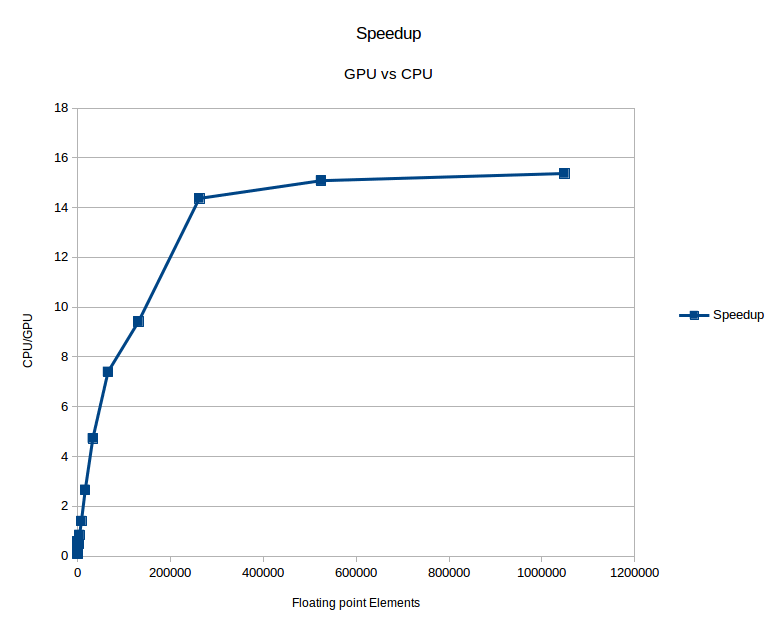
\includegraphics[width=8.5cm]{speedup.png}      
  \caption{GPU Speedup Graph.}
  \label{fig:speedup}
\end{figure}
Overall the GPU outperforms the CPU when N is large and peaks at around a 15x performance increase over the CPU as seen in figure~\ref{fig:speedup}.
\begin{table}
{%
\newcommand{\mc}[3]{\multicolumn{#1}{#2}{#3}}
\begin{center}
\begin{tabular}[t]{|l|lll}\hline
\mc{4}{|c|}{Best Results}\\\hline
N                         & \mc{1}{l|}{CPU RECALL}& \mc{1}{l|}{GPU RECALL}& \mc{1}{l|}{Speed-up}    \\\hline
\mc{1}{|r|}{2048}         & \mc{1}{r|}{0.0418304} & \mc{1}{r|}{0.0408192} & \mc{1}{r|}{1.024772656} \\\hline
\mc{1}{|r|}{8192}         & \mc{1}{r|}{0.0519552} & \mc{1}{r|}{0.0503296} & \mc{1}{r|}{1.032299084} \\\hline
\mc{1}{|r|}{262144}       & \mc{1}{r|}{0.3347328} & \mc{1}{r|}{0.3425152} & \mc{1}{r|}{0.9772786726}\\\hline
\mc{1}{|r|}{524288}       & \mc{1}{r|}{0.5480384} & \mc{1}{r|}{0.5567296} & \mc{1}{r|}{0.9843888308}\\\hline
\mc{1}{|r|}{1048576}      & \mc{1}{r|}{0.884032}  & \mc{1}{r|}{0.8959488} & \mc{1}{r|}{0.98669924}  \\\hline
\mc{1}{|r|}{10000000}     & \mc{1}{r|}{6.2174528} & \mc{1}{r|}{6.2613952} & \mc{1}{r|}{0.9929820114}\\\hline
\end{tabular}
\end{center}
}%
\caption{Fastest run-times recorded for each vector size.}
\label{tab:best}
\end{table}

\begin{figure}[!t]
  \centering
  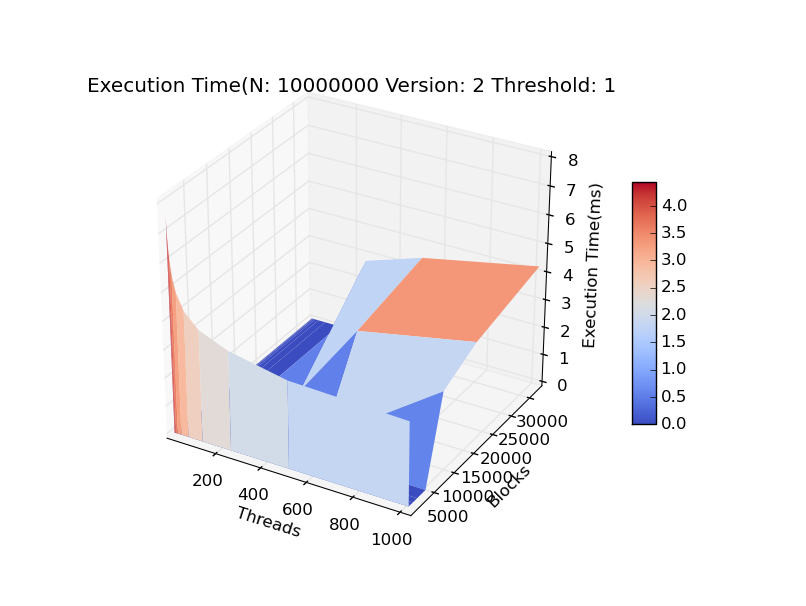
\includegraphics[width=8.5cm]{figure_12.png}      
  \caption{GPU Kernel Recall: Unstable calls result in a zero run-time.}
  \label{fig:unstable}
\end{figure}


\begin{figure}[!t]
  \centering
  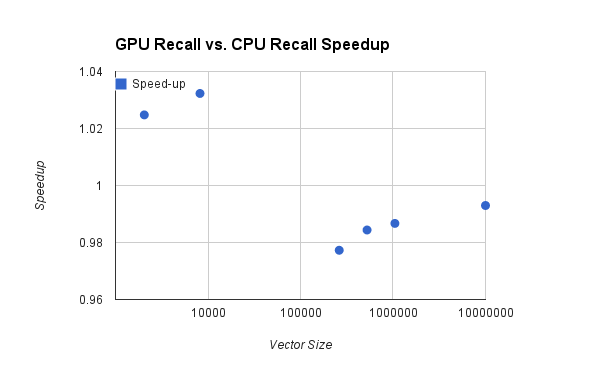
\includegraphics[width=8.5cm]{speeduprecall.png}      
  \caption{GPU/CPU Recall Speedup Graph.}
  \label{fig:recallspeedup}
\end{figure}

\begin{figure}[!t]
  \centering
  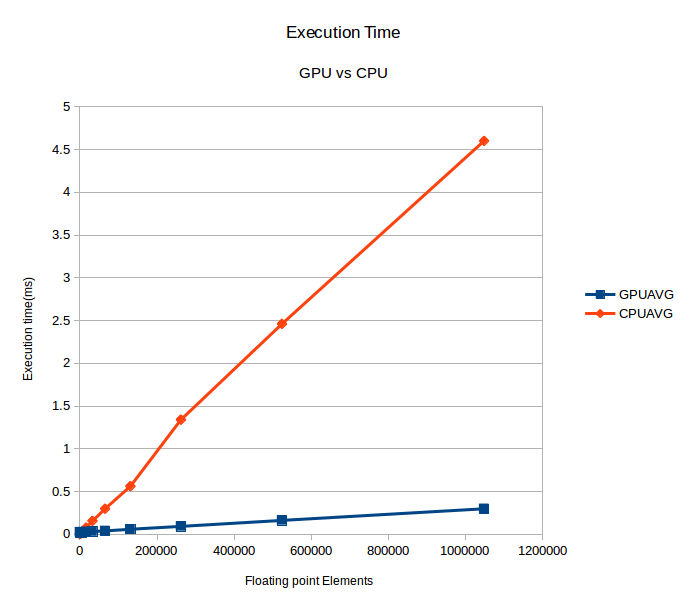
\includegraphics[width=8.5cm]{execution_time.png}      
  \caption{GPU/CPU Execution time.}
  \label{fig:execute}
\end{figure}

\begin{figure}[!t]
  \centering
  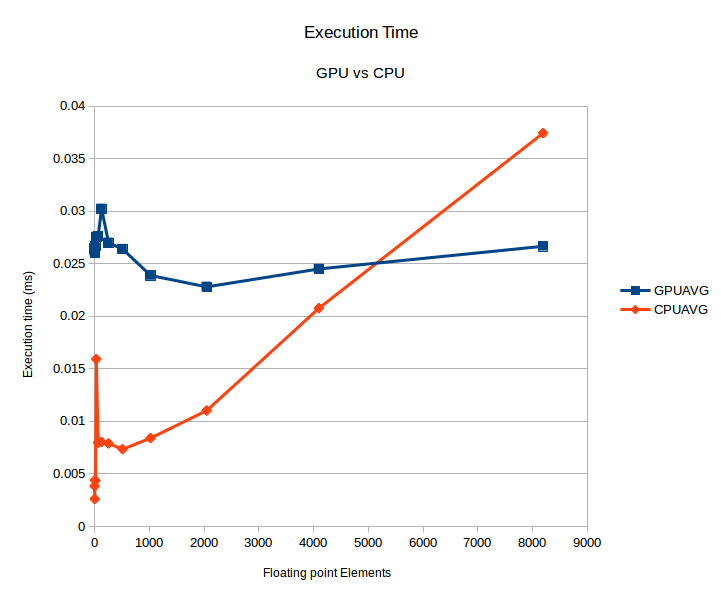
\includegraphics[width=8.5cm]{execution_time_short.png}      
  \caption{GPU/CPU Execution time Short.}
  \label{fig:executeshort}
\end{figure}

\begin{figure}[!t]
  \centering
  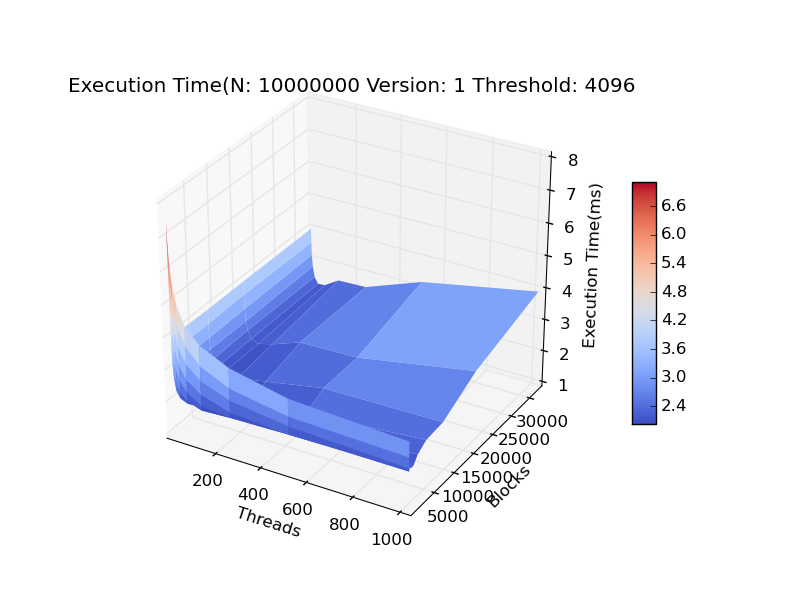
\includegraphics[width=8.5cm]{figure_10.png}      
  \caption{GPU Execution time. N=100,000,000}
  \label{fig:}
\end{figure}

\begin{figure}[!t]
  \centering
  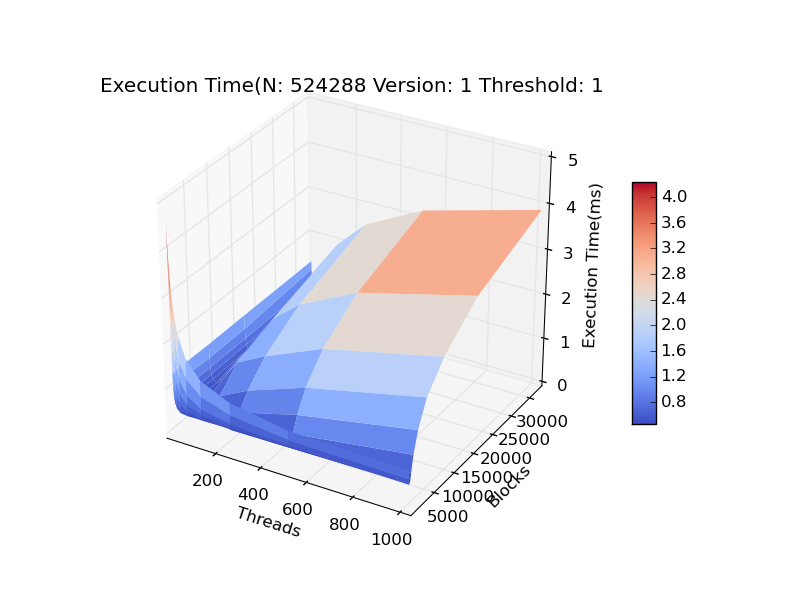
\includegraphics[width=8.5cm]{figure_5.png}      
  \caption{GPU Execution time. N=524,288}
  \label{fig:n524288v1}
\end{figure}

% An example of a double column floating figure using two subfigures.
% (The subfig.sty package must be loaded for this to work.)
% The subfigure \label commands are set within each subfloat command,
% and the \label for the overall figure must come after \caption.
% \hfil is used as a separator to get equal spacing.
% Watch out that the combined width of all the subfigures on a 
% line do not exceed the text width or a line break will occur.
%
%\begin{figure*}[!t]
%\centering
%\subfloat[Case I]{\includegraphics[width=2.5in]{box}%
%\label{fig_first_case}}
%\hfil
%\subfloat[Case II]{\includegraphics[width=2.5in]{box}%
%\label{fig_second_case}}
%\caption{Simulation results for the network.}
%\label{fig_sim}
%\end{figure*}
%
% Note that often IEEE papers with subfigures do not employ subfigure
% captions (using the optional argument to \subfloat[]), but instead will
% reference/describe all of them (a), (b), etc., within the main caption.
% Be aware that for subfig.sty to generate the (a), (b), etc., subfigure
% labels, the optional argument to \subfloat must be present. If a
% subcaption is not desired, just leave its contents blank,
% e.g., \subfloat[].


% An example of a floating table. Note that, for IEEE style tables, the
% \caption command should come BEFORE the table and, given that table
% captions serve much like titles, are usually capitalized except for words
% such as a, an, and, as, at, but, by, for, in, nor, of, on, or, the, to
% and up, which are usually not capitalized unless they are the first or
% last word of the caption. Table text will default to \footnotesize as
% IEEE normally uses this smaller font for tables.
% The \label must come after \caption as always.
%
%\begin{table}[!t]
%% increase table row spacing, adjust to taste
%\renewcommand{\arraystretch}{1.3}
% if using array.sty, it might be a good idea to tweak the value of
% \extrarowheight as needed to properly center the text within the cells
%\caption{An Example of a Table}
%\label{table_example}
%\centering
%% Some packages, such as MDW tools, offer better commands for making tables
%% than the plain LaTeX2e tabular which is used here.
%\begin{tabular}{|c||c|}
%\hline
%One & Two\\
%\hline
%Three & Four\\
%\hline
%\end{tabular}
%\end{table}

% \section{Conclusion}
% The conclusion goes here.

\bibliographystyle{IEEEtran}
%\bibliography{IEEEabrv,../bib/paper}
%\bibliographystyle{plain}
%\bibliography{IEEEabrv, references}
\end{document}


